%%
%%
%%  complexity_featureselection.tex
%%
%%
%%%%%%%%%%%%%%%%%%%%%%%%%%%%%%%%%%%%%%%%%
%%                                     %%
%%  				       %%
%%     				       %%
%%                                     %%
%%         < ?? Agosto 2009 >          %%
%%                                     %%
%%                                     %%
%%                                     %%
%%%%%%%%%%%%%%%%%%%%%%%%%%%%%%%%%%%%%%%%%



\NeedsTeXFormat{LaTeX2e}[1995/12/01]
\documentclass[10pt]{bmc_article}



% Load packages
\usepackage{cite} % Make references as [1-4], not [1,2,3,4]
\usepackage{url}  % Formatting web addresses
\usepackage{ifthen}  % Conditional
\usepackage{multicol}   %Columns
\usepackage{graphicx}
\usepackage[utf8]{inputenc} %unicode support
%\usepackage[applemac]{inputenc} %applemac support if unicode package fails
%\usepackage[latin1]{inputenc} %UNIX support if unicode package fails
\urlstyle{rm}


%%%%%%%%%%%%%%%%%%%%%%%%%%%%%%%%%%%%%%%%%%%%%%%%%	
%%                                             %%
%%  If you wish to display your graphics for   %%
%%  your own use using includegraphic or       %%
%%  includegraphics, then comment out the      %%
%%  following two lines of code.               %%
%%  NB: These line *must* be included when     %%
%%  submitting to BMC.                         %%
%%  All figure files must be submitted as      %%
%%  separate graphics through the BMC          %%
%%  submission process, not included in the    %%
%%  submitted article.                         %%
%%                                             %%
%%%%%%%%%%%%%%%%%%%%%%%%%%%%%%%%%%%%%%%%%%%%%%%%%


%\def\includegraphic{}
%\def\includegraphics{}



\setlength{\topmargin}{0.0cm}
\setlength{\textheight}{21.5cm}
\setlength{\oddsidemargin}{0cm}
\setlength{\textwidth}{16.5cm}
\setlength{\columnsep}{0.6cm}

\newboolean{publ}

%%%%%%%%%%%%%%%%%%%%%%%%%%%%%%%%%%%%%%%%%%%%%%%%%%
%%                                              %%
%% You may change the following style settings  %%
%% Should you wish to format your article       %%
%% in a publication style for printing out and  %%
%% sharing with colleagues, but ensure that     %%
%% before submitting to BMC that the style is   %%
%% returned to the Review style setting.        %%
%%                                              %%
%%%%%%%%%%%%%%%%%%%%%%%%%%%%%%%%%%%%%%%%%%%%%%%%%%


%Review style settings
\newenvironment{bmcformat}{\begin{raggedright}\baselineskip20pt\sloppy\setboolean{publ}{false}}{\end{raggedright}\baselineskip20pt\sloppy}

%Publication style settings
%\newenvironment{bmcformat}{\fussy\setboolean{publ}{true}}{\fussy}



% Begin ...
\begin{document}
\begin{bmcformat}


%%%%%%%%%%%%%%%%%%%%%%%%%%%%%%%%%%%%%%%%%%%%%%
%%                                          %%
%% Enter the title of your article here     %%
%%                                          %%
%%%%%%%%%%%%%%%%%%%%%%%%%%%%%%%%%%%%%%%%%%%%%%

\title{Classification Complexity in Gene Marker Discovery: analysis on cancer gene expression data}

%%%%%%%%%%%%%%%%%%%%%%%%%%%%%%%%%%%%%%%%%%%%%%
%%                                          %%
%% Enter the authors here                   %%
%%                                          %%
%% Ensure \and is entered between all but   %%
%% the last two authors. This will be       %%
%% replaced by a comma in the final article %%
%%                                          %%
%% Ensure there are no trailing spaces at   %%
%% the ends of the lines                    %%     	
%%                                          %%
%%%%%%%%%%%%%%%%%%%%%%%%%%%%%%%%%%%%%%%%%%%%%%


\author{Ivan G. Costa\correspondingauthor$^1$%
       \email{IGC\correspondingauthor - igcf@cin.ufpe.br}%
      \and
         Thais G. do Rego $^1$%
         \email{TGR - tgr2@cin.ufpe.br}
      \and
         Clerton R. A. Filho$^1$%
         \email{CRAF - craf@cin.ufpe.br}
      \and
         Eduardo G. Gusmao$^1$%
         \email{EGG - egg@cin.ufpe.br}
       and
         Ana C. Lorena$^{2}$ \email{ACL - ana.lorena@ufabc.edu.br}
       and
         Marcilio C. P. de Souto$^{3}$ \email{MCPS - marcilio@dimap.ufrn.br}
      }

% XXX - clerton - decidir nome

%%%%%%%%%%%%%%%%%%%%%%%%%%%%%%%%%%%%%%%%%%%%%%
%%                                          %%
%% Enter the authors' addresses here        %%
%%                                          %%
%%%%%%%%%%%%%%%%%%%%%%%%%%%%%%%%%%%%%%%%%%%%%%

\address{
    \iid(1) Center of Informatics, Federal University of Pernambuco, Brazil\\
    \iid(2) Center of Mathematics, Computation and Cognition, ABC Fed. Univ., SP, Brazil\\
    \iid(3) Dept. of Informatics and Applied Mathematics, Fed. Univ. of Rio Grande do Norte, Brazil
}

\maketitle

%%%%%%%%%%%%%%%%%%%%%%%%%%%%%%%%%%%%%%%%%%%%%%
%%                                          %%
%% The Abstract begins here                 %%
%%                                          %%
%% The Section headings here are those for  %%
%% a Research article submitted to a        %%
%% BMC-Series journal.                      %%
%%                                          %%
%% If your article is not of this type,     %%
%% then refer to the Instructions for       %%
%% authors on http://www.biomedcentral.com  %%
%% and change the section headings          %%
%% accordingly.                             %%
%%                                          %%
%%%%%%%%%%%%%%%%%%%%%%%%%%%%%%%%%%%%%%%%%%%%%%


\begin{abstract}

\paragraph*{Background:}

Classification methods are the main methodology for performing
diagnosis and gene marker selection from expression profiles of cancer
patients. Nevertheless, gene expression data pose several challenges
for these methods. For example, there are high numbers of genes, few
patient samples and, in addition, expression values can have noise.

        \paragraph*{Results:}

We investigate th suitability of certain statistical indices that measure aspects
such as data geometry, topology and complexity of classification
boundary to indicate the difficulty in performing classification and
gene marker selection in a particular cancer diagnosis data sets. In
order to do so, we study the correlation of these indices to the
performance of several classification/gene marker selection methods
such as SVM, shrunken centroids, discriminant analysis and KNN for
several cancer gene expression data sets.

        \paragraph*{Conclusions:}

These analysis allow us to investigate the relation of some of the
complexity indices in explaining the difficulty of performing cancer
diagnosis and marker selection. Therefore, it helps the understanding how the
characteristics of these data sets influence the performance of common
classification and gene selection methods employed in the
literature. Furthermore, some of the indices have a potential to
support the selection of a diagnostic/marker methodology for a
particular data set.



\end{abstract}



\ifthenelse{\boolean{publ}}{\begin{multicols}{2}}{}




%%%%%%%%%%%%%%%%%%%%%%%%%%%%%%%%%%%%%%%%%%%%%%
%%                                          %%
%% The Main Body begins here                %%
%%                                          %%
%% The Section headings here are those for  %%
%% a Research article submitted to a        %%
%% BMC-Series journal.                      %%
%%                                          %%
%% If your article is not of this type,     %%
%% then refer to the instructions for       %%
%% authors on:                              %%
%% http://www.biomedcentral.com/info/authors%%
%% and change the section headings          %%
%% accordingly.                             %%
%%                                          %%
%% See the Results and Discussion section   %%
%% for details on how to create sub-sections%%
%%                                          %%
%% use \cite{...} to cite references        %%
%%  \cite{koon} and                         %%
%%  \cite{oreg,khar,zvai,xjon,schn,pond}    %%
%%  \nocite{smith,marg,hunn,advi,koha,mouse}%%
%%                                          %%
%%%%%%%%%%%%%%%%%%%%%%%%%%%%%%%%%%%%%%%%%%%%%%




%%%%%%%%%%%%%%%%
%% Background %%
%%
\section*{Background}

The measurement of genome-wide expression of patients allows clinical
diagnosis to be performed in a molecular
level~\cite{Spang2003,Veer2008}. Given a set of patient expression
profiles and its diagnosis, we can use classification methods to find
models able to diagnose a new oncoming patient based only on his/her
expression profile~\cite{Spang2003}. Nevertheless, characteristics of
gene expression data often makes the task of diagnosis hard. These
data sets usually have few patients and measure the expression values
of thousands of genes, making the classification problem to lie in a
high-dimensional and sparse space. Furthermore, gene expression data
have missing values, suffer from several sources of noise and includes
patient variability~\cite{Irizarry2005}.

One important aspect of classification methods is the selection of a
subset of genes, whose expression are mostly discriminative for
performing the diagnosis of a particular disease. These gene markers
could give insights on the molecular mechanisms of the
disease. Furthermore, they can be used with small scale profiling
technologies, thus enabling the creation of cheap, reliable and easy
to perform diagnostic tests~\cite{Veer2008}. From a methodological
point of view, gene selection (or feature selection) could improve the
classification error by drastically reducing the gene expression
data space. Therefore, data sparsity is lowered and classifiers could
have a better generalization in classifying new
patients~\cite{Song2007}.

We have previously performed a study on cancer gene expression data in
which we measured statistics of data geometry, topology and shape of
the classification boundary to indicate the complexity of the
classification task for a given data set~\cite{Costa2009b}.  In order
to do so, we used a selection of seven classification complexity
indices proposed in~\cite{Ho2002} for general classification problems
(see Figure~1 for an example of these complexity statistics). Then, we
performed classification using four classical methods considering 10
different gene expression data sets. We found that two complexity
indices, Mixture Identifiability and Dimensionality/Sample ratio, were
correlated with the test error rates of all classification methods
analyzed. In particular, the correlation with the
Dimensionality/Sample ratio indicated that the sparsity of the data
space is a major aspect in indicating complexity of gene
expression-based classification.

In the current work, we extend our previous study by, among other
things, performing gene marker selection prior to cancer
classification. We employed two gene selection methods, which have been
already used in gene expression analysis: sum of squared distances
between classes divided by the sum of squares distances within classes
(BSS/WSS) and Fisher ratio~\cite{Dudoit2002}; and four popular
classification methods: Support Vector Machine
(SVM)~\cite{Vapnik1995}, Diagonal Discriminant Analysis
(DDA)~\cite{Hastie2001}, k-nearest neighbor (KNN)~\cite{Ripley1996}
and Shrunken centroids~\cite{Tibshirani2002}. Furthermore, we use
additional data sets to increase the statistical power of our
analysis. 

We aim to investigate the relation of the complexity indices in
explaining the difficulty in performing cancer diagnosis together with
gene marker selection. By doing so, we intend to gain insights on the
performance of these classification and gene selection techniques,
when they are presented to data sets with particular complexity
characteristics.  Furthermore, we would like to explore, which indices
have a potential to support the selection of a diagnostic/gene
selection methodology for a particular data set.


%%%%%%%%%%%%%%%%%%%%%%%%%%%%
%% Results and Discussion %%
%%
\section*{Results and Discussion}

\subsection*{Comparative Analysis}

We performed classification using Shrunken Centroids, SVM, KNN and DDA
classifiers with the two feature selection methodologies - SSW/SSB and
Fisher Ratio - for the gene expression data bases described in
Table~1. Given that SVMs and most of the complexity indices are only
able to be employed in classification problems with two classes, we
performed one-against-all decompositions for each data set, in which
for a problem with $C$ classes, $C$ subproblems are generated, each
one distinguishing one class from the remaining classes. This resulted
in 85 decomposed data sets. The use of such a decomposition strategy
has been indicated in studies analyzing the problem of multi-class
classification with SVMs as often leading to overall best classification of
cancer gene expression data~\cite{Statnikov2005}.

For each combination of classification method, gene selection
technique and data set decomposition, we performed leave-one-out
cross-validation, and measured test error. Feature selection was then
performed by a nested cross-validation, selecting for each training
data set the top 500, 250, 100, 50, 25 and 10 genes. The Shrunken
Centroids method, which automatically performs feature selection, used
only data without feature selection. In the end, we kept the best test
error and the number of selected genes of a classification method on a
data set. These results can be seen in Additional Material~1. More
details of the feature selection procedures, classification methods
and complexity indices employed are described in the Section
``Methods''.

\subsection*{Classification Error}

The performance of the classifiers can be seen in the Additional
Material~1. Overall, Shrunken Centroids and SVM with/without feature
selection obtained the lowest classification test errors for most of
the data sets: respectively, 33 and 40 out of 85 data sets. In relation
to the use of feature selection, 18 of the lowest classification
errors were obtained when no feature selection was performed; 20 used
the BSS/WSS technique; 7 the Fisher ratio technique and 40 with
Shrunken Centroids. These results indicate that in the majority of
cases (67 out of 85), classification error was lowered after feature
selection.

% shrunken centroids como normal ...

\subsection*{Classification Complexity}

% tirar accuracy -> por error
% checar legenda
% por tt

Our main concern here is to compare the error rate of these
classifiers generated with the complexity indices describing the
data. These results are summarized in Figure~2. This figure presents
scatter plots of the complexity indices (y-axis) versus classification
error (x-axis) for classification and feature selection methods (see
Section ``Methods'' for a description of the complexity indices). At
each plot, points represent the 85 one-against-all decompositions of
the data sets. For each method, {\tt 1} stands for no feature
selection, {\tt 2} for BSS/WSS and {\tt 3} for Fisher ratio. Numbers
in the left upper corner of each scatter plot correspond to the
correlation between the error rate and complexity indices. Red values
indicate correlations that are statistically significant ($t$-test
with $p$-value $< 0.01$).

Two complexity indices measuring linear separability (L1 and L2) have
values equal or very close to zero for all data sets (data not
shown). This indicates that the high dimensionality makes data to be
linearly separable in all ``one-against-all'' decompositions. Another
index that had little discriminative power indicating classification
complexity is F2, which measures class overlap. The values of this
index were low for most of the data sets, indicating that there is
little overlap between classes. The low overlap is likely a result
of the data sparsity induced by the high dimensionality of the data
sets. We would like to stress that we modified the definition of F2,
as it contained a conceptual error in the original
definition~\cite{Ho2002}. See Section Methods for details.

% explicitar que f2 foi modificado.

The indices N1, N2 and N3 displayed the most significant correlation
with all methods and feature selection techniques with the exception
of DDA with Fisher ratio. The positive correlation values evidence
that higher values of these indices lead to higher error rates, which
indicate more difficult classification problems. Therefore, these
indices, which are based on very simple distance based measures, do
indeed capture most of the information regarding classification
complexity. Still regarding the indices N1, N2 and N3, we can observe
that SVM and DDA with the BSS/WSS feature selection presented higher
correlations than the other cases. This indicates that the error rate
of this feature selection method is more correlated with the data set
complexity described by these particular indices.

Another relevant index is $log(D)$, which captures the dimensionality
of the original data set previously from feature selection. In this
case, the relation with the classification error rate was inverse,
that is, high dimensions usually implicated in lower classification
error rates. We estimated a similar index $log(D')$, where $D'$ is the
number of genes indicated by the feature selection procedure. In this
scenario (data not shown), no correlation was found.  This indicates
that a higher number of genes in the original data set leads
classifiers to obtain lower classification errors. On the other hand,
we found no relation between classification complexity and the number
of genes after feature selection was performed.


%- ANA: ESSA FRASE EST CONTRADIZENDO A ANTERIOR. DEVERIA SER LOWER
%CLASSIFICATION ERRORS. O QUE PEGA EM CONCLUIR ISSO  QUE ENTO PODEM
%DIZER QUE: ENTO NO VALE A PENA FAZER FEATURE SELECTION? - CLARO QUE
%FEATURE SELECTION TB  PARA IDENTIFICAR GENES CANDIDATOS - OU: O
%FEATURE SELECTION VAI DIMINUIR A DIMENSO E A VOC TER MAIOR ERRO? 
%EU ACHO QUE ESSAS CONCLUSES DEVEM SER REVISTAS E MELHOR EXPLICADAS}

% oi, o texto acima estava mal escrito.juntei o paragrafo abaixo. Sim, vale a pena fazer feature selection,isto ja e mostrado pela melhora geral dos resultados. O que digo acima  que o numero de genes finais nao indica complexidade.

%We also measured if there was a relation between the number of genes
%selected by the feature selection and the classification
%complexity. However, there was no significant correlation of the
%number of genes with the complexity indices. This indicates that
%although methods mostly profited from feature selection \textbf{ANA:
%BASEADO EM QUE? ERRO?}, we could not find any relation of the number
%of genes or classification error \textbf{ANA: ONDE ENTROU CORRELAO
%COM CLASSIFICATION ERROR NESSA ANLISE? NO FOI S O NMERO DE GENES?} 
%to the complexity indices.

Lower F1 values indicate more complex classification problems. The
plots show an increase in the error rates with lower F1
values. However, this index did not present a significantly high
correlation to many methods. Furthermore, only KNN and SVM
with/without feature selection showed positive correlation with the T1
index, which indicates that the dimensionality/number of sample ratios
are critical to these classifiers, but not to DDA and Shrunken
centroid.

To check if we could combine these indices in a linear manner, we
applied principal component analysis to the indices, and included the
1st component as a complexity index. This component represents 67$\%$
of the variance in the data. As seen in Figure~2, this index had a
high correlation with all methods, except from DDA and Fisher
ratio. The correlation of the 1st PCA was similar to the correlation
of N1, N2 and N3. 

%This sugests that most of the classification complexity is already measured by N1, N2 and N3.

The results presented here are compatible with the ones from our
previous study~\cite{Costa2009b}. There N1 and T1 displayed
significant correlation with KNN, SVM and other methods. Similar
results were observed in the current work, but because of the increase
in the number of data sets and complexity indices, we detected here
significant correlation of these methods with other complexity indices
as well.

%\textbf{ ANA: SERIA INTERESSANTE COLOCAR A OBSERVAO DO MARCILIO QUANDO A CORRELAO DO KNN COM OS INDICES N2 E N3. ALIS, PR%INCIPALMENTE O N3. ME PARECE ESTRANHO A PRINCPIO RELACIONAR ERRO EM LOO COM ERRO EM LOO DE NOVO,  MUITO PROVVEL QUE SERO C%ORRELACIONADOS - PRINCIPALMENTE PARA A MESMA TCNICA - PARA OUTRAS, MEDE UM POUCO O QUANTO ELAS CONCORDAM. MAS A PRINCPIO POD%ERIA USAR ENTO QUALQUER OUTRA TCNICA DE AM PARA DAR UM INDICE DE COMPLEXIDADE. O ERRO  UMA BOA MEDIDA DE COMPLEXIDADE? EM G%ERAL SIM, MAIOR ERRO, MAIOR COMPLEXIDADE. MAS E QUANDO SE TEM OVERFITTING? O DATA SET PODE SER SUPER SIMPLES E O FATO  QUE SE% USOU UM CLASSIFICADOR COMPLEXO NELE}

% Ok, concordo que na verdade KNN nao precisaria estar neste estudo. Na verdade so o N3  um classificador por si so, mas um bem simples, nao parametricos e que nao tem problemas de overfitting (KNN com K alto  uma tecnicas com baixissimo vies, logo pouco sucetivel a overfiting). Na verdade, inclui erronalmente esta frase anteriormente (dizendo que N1 e N2 tambem eram classificadores por si soh).

% DDA 3 has somehow strange results... CONCORDO, ESTÁ ESTRANHO, FOGE DE TUDO
% XXX Ivan - vou re-rodar ele e checar a implementação.
% XXX - rerodei o dda e nao achei nada 


%%%%%%%%%%%%%%%%%%%%%%
\section*{Conclusions}


The experimental results obtained in this analysis lead us to the
following conclusions. The classification complexity indices N1, N2
and N3 successfully explained classification complexity regardless of
the method or feature selection used. Another relevant complexity
index is the log of the number of genes in the original data set. This
indicates that all methods, except DDA, profit from a higher number of
genes to perform accurate classification. This suggests that studies
of microarray based diagnosis do profit from a larger coverage of
genes included in the microarrays. Furthermore, most methods are
sensible for the index T1, which measures the ratio between number of
genes/number of samples. Thus, a low number of patients and the high
dimension of the data sets is another factor limiting the accuracy of
these classification methods.

%\textbf{ANA: NO SEI
%BEM O QUE DIZER NESTE CASO, ME PARECE ARRISCADO DIZER QUE SHOULD BE
%AVOIDED. TALVEZ FOSSE MELHOR DIZER QUE ELES PARECEM MAIS SENSVEIS A
%DATA SETS COM MUITAS DIMENSES E POUCOS EXEMPLOS.  QUE EM TEXT MINING
%O PESSOAL COSTUMA PREFERIR SVM QUANDO SE TEM POUCOS EXEMPLOS, E 
%JUSTAMENTE UM DOMNIO EM QUE SE TEM TB MUITOS ATRIBUTOS...}
% sera que o naive e o shrunken  melhor para dimensoes altas ...

Some findings are in accordance with common knowledge from the gene
expression literature, but not yet studied in such large scale
expression compendia. First, all data sets decompositions are linearly
decomposable, as previously observed in~\cite{Lorena2008}. In relation
to the use feature selection, we could see an overall improvement of
error rates in $83\%$ of the data sets, as previously observed
before~\cite{Song2007,Statnikov2005,Tibshirani2002}. However, we found
no relation between the complexity indices, number of genes selected
or error rates. This indicates that there is no direct relationship
between the error improvement after feature selection and the
classification complexity indices used in this study.

%\end{itemize}


%\textbf{PONTOS A DISCUTIR:}
%
%\begin{itemize}
%\item - DEU PARA ENTENDER COMO A COMPLEXIDADE DOS DADOS INFLUENCIA NO DESEMPENHO DOS MÉTODOS? PARA ISSO SERIA IMPORTANTE AVALIAR OS RESULTADOS FRENTE AO QUE CADA UM DOS ÍNDICES MEDE EM ESPECÍFICO;
%Sim. Os fatos de BSS/WSS terem maior correlação com N1, N2, N3 e de SVM e KNN serem mais correlacionamos com T1. Mas concordo com a musa que a correlação (ou a sua falta) não é o melhor jeito de fazer isto.
%\item - DÁ PARA TIRAR ALGUMA CONCLUSÃO SE REALMENTE FAZER FEATURE SELECTION MELHORA A COMPLEXIDADE DO PROBLEMA DE CLASSIFICAÇÃO RESOLVIDO? E ENTRE OS DOIS MÉTODOS DE SELEÇÃO, ALGUM PODE SER CONSIDERADO MELHOR NESSE ASPECTO?
%nem sempre. Obviamente no geral o shrunken e o svm com feature foram melhores, mas em algunas casos svm sem filtro tb foi ol.
%\item - OS RESULTADOS FORAM PARECIDOS COM OS QUE JÁ TIVEMOS?
%Sim, a analise dos metodos com 1 sao equivalentes ao que tentamos inicialmente.
%\item - DÁ PARA REALMENTE RECOMENDAR ALGUMA TÉCNICA OLHANDO OS RESULTADOS DOS ÍNDICES? COMO?
%Isso aqui so com metalearning - a gente precisa de metalearning aqui. Dei uma olhada nos grafico
%\end{itemize}



%%%%%%%%%%%%%%%%%%
\section*{Methods}

\subsection*{Data}

The data of microarray experiments used in this work were collected in
GEO (\emph{Gene Expression Omnibus})~\cite{Barret2007} or in existing
literature. These data sets, which are based on either cDNA or
Affymetrix platforms, are a selection of data sets
from~\cite{Souto2008}. The final list of data sets, along with their
number of patients, type of microarray platform, class distributions
and number of genes are described in Table~1.

We introduce here the basic notation used to describe the cancer gene
expression data. Let  $X$ be a $n$ by $d$ matrix representing a gene
expression data set, where $x_{ij}$ denotes the expression value of
sample $i$ and feature (gene) $j$, $x_i$ is a $d$-dimensional vector with the
expression values of sample (patient) $i$ and $x_{.j}$ is a
$n$-dimensional vector representing the expression values of feature
(gene) $j$. Moreover, $Y$ is an $n$-dimensional vector, where $y_i \in
\{1,..,C\}$ corresponds to the class (or cancer type) of patient $i$ and
$C$ is the total number of classes (cancer types) in the data set.

As previously discussed, for data sets with more than 2 classes, we
performed one-against all decomposition.  That is, for a particular
class $k$, we created a new class vector $Y^k$, where $y^k_i=1$ if
sample $i$ belongs to class $k$ in the original classification
($y_i=k$) and $y^k_i=0$ otherwise ($y_i\neq k$). Thus, we obtain $C$
decompositions of data sets, where $C$ is larger than 2.


\subsection*{Pre-processing and Unsupervised Filtering}

We apply an unsupervised filter to discard missing values and genes
displaying no differential expression within the patients. This
filtering, which works without the class information, was applied as
in~\cite{Souto2008}.  The pre-processing performed on data from
experiments based on the Affymetrix platform has the following steps:
(1) values below 10 and above 16000 have been replaced by these
bounds, (2) we measure the mean expression of $x_{.j}$, which is
represented by $\overline{x}_{.j}$ and eliminate 10$\%$ of the highest
and lowest values to avoid extreme values (3) each $x_{ij}$ is
replaced by $x\prime_{ij} = \log_2 (x_{ij}/\overline{x}_{.j})$. In
cDNA platform data, it was not necessary to apply transformations, as
they were already in logarithmic scale. However, they required the
handling of missing values. We eliminated genes that showed more than
10$\%$ of missing values. The remaining missing values were
substituted by the average expression values of the genes through all
tissues. The unsupervised filter process was as follows: two $l$ and
$c$ thresholds were chosen, where the absolute value of the feature
$x_{.j}$ has to be higher than $l$ in at least $c$ patients. Genes
that do not obey this restriction were excluded from the data
set. Column ``d'' in Table~1 shows the numbers of genes remaining in
the data sets after the employment of the former pre-processing and
filtering steps.

\subsection*{Supervised Filter}

In marker selection, one of the main aspects is the use of statistics
to select features (or genes) which best discriminate the classes of
patients. We inspect in this work two simple feature selection
procedures, which have been successfully applied in previous gene expression
studies~\cite{Dudoit2002}.

The first measure is the sum of squares of squared distances between
groups divided by the sum of squares within groups. For feature
(gene) $j$, this measure is:

\begin{equation}
BSS/WSS(j) = \frac{\sum^n_i\sum^C_k I(y_i = k)(\overline{x}^k_{.j} -
\overline{x}{_.}{_j}){^2}} {\sum^n_i\sum^C_k I(y_i =
k)(x{_i}{_j} -\overline{x}^k_{.j}){^2}}
\end{equation}

where $\overline{x}_.$$_j$ represents the average level of expression
of gene $j$ among all samples and $\overline{x}^k_{.j}$ represents the
average level of expression of gene $j$ among the samples belonging to
class $k$.


We also use the filter using the Fisher ratio (FR), a measure for
(linear) discriminative power of some variable, which is defined as:

%\textbf{A equação abaixo é na verdade a rigor a mesma do índice F1, certo? - é o discriminante de Fisher. Acho que seria melhor deixar %com notação parecida, pois está diferente. Aliás, lá está com a variância embaixo, aqui está com o desvio-padrão. Também pensando no negócio da correlação. O índice F1 máximo do índice de Fisher entre todos os atributos. E a seleção de features por Fisher pega os k com %maior valor de índice de Fisher. Não deveria haver alguma correlação então dos de seleção de atributos com Fisher em relação a F1?}

% XXX - ivan - as equacoes sao parecidas (na verdade F1 é o maximo de todos os valores), mas eles sao usados em contextos bem diferentes (selecao de genes X complexidade de base). Sim, deveria haver uma relacao, mas nao tao direta assim.

\begin{equation}
FR = \frac{\overline{x}^{(1)}_{.j} - \overline{x}^{(2)}_{.j}}{\sigma^{2(1)}_{j} +\sigma^{2(2)}_{j} }
\end{equation}
where $\overline{x}^{(k)}_{.j}$ is the mean of feature $j$ in class
$k$ and $\sigma^{2(k)}_{j}$ is the variance of the class $k$ for
feature $j$~\cite{Peng2006}.  For both feature selection indices, we
select the $p$ genes with highest values from a particular training
data set to perform classification experiments~\cite{Dudoit2002}.

\subsection*{Classification Methods}

Four classification methods were used for supervised classification in
our study: K-nearest neighbors (KNN), support vector machines (SVM),
diagonal discriminant analysis (DDA) and nearest shrunken centroid
(NSC).\\

{\bf K-nearest neighbors} (KNN) algorithm is a method that classifies
samples based on the classes of their $k$ nearest samples in the
training data~\cite{Ripley1996}. Here, we used the Euclidean distance
to find the closest neighbors and set the parameter $k=3$.\\

{\bf Support Vector Machines} (SVMs) is a classification method based
on statistical learning theory~\cite{Vapnik1995}.  Given a dataset,
SVMs finds a hyperplane dividing the samples from two classes while
also maximizing the distance of these samples to the hyperplane. In
particular, we use a Sequential Minimal Optimization (SMO) method for
inducing the SVMs implemented in Weka~\cite{WIT05}. As indicated in
previous studies, most gene expression cancer data sets are linearly
separable~\cite{Lorena2008}, thus we use simple linear SVMs in our
experiments. All other parameters are set as default, as given in the
software Weka. It should be also noticed that the SVMs original
formulation tackles with binary classification problems. An
one-against-all decomposition was employed for multi-class
classification.\\

{\bf Diagonal discriminant analysis} (DDA) method is based on the use
of Gaussians distributions as discriminant rule for
classification. Here, we used Gaussians with diagonal class covariance
matrices, which assumes independence between
features~\cite{Dudoit2002}. This method requires no selection of
parameters. We used for this method an implementation in the R
SMA (Statistics for Microarray Analysis) package.


{\bf Nearest Shrunken centroids} is a method for centroid based
classification, which performs automatic feature
selection~\cite{Tibshirani2002}. The feature selection is based on
shrinking centroids of particular features that have a low
discrimination power between the classes. The shrinkage factor
$\Delta$ controls the stringency of the shrinkage factor and set some
of the class centroids of particular genes equally, thus
discarding these genes from the classifier. For these experiments, we
used a nested cross-validation procedure to select the parameter
$\Delta$, as implemented in the PAMR (Prediction Analysis for Microarrays
in R) package.\\

In all these methodologies, the final classifier test error was measured
with a leave-one-out procedure. Moreover, feature selection was
performed in the training data only, to avoid the introduction of bias
in the results.

\subsection*{Classification Complexity Measures}

We used a selection of indices proposed in~\cite{Ho2002} and used
in~\cite{Costa2009b} to measure classification complexity. Most of
these indices are by design only able for accessing data sets with two
classes. Therefore, we measure then using a one against all decomposition of
the data sets.

We also include in this study a novel complexity index that measures
the number of dimensions, which contains most variance in the
data. Moreover, we also propose a modification of the Volume
of Overlapping Region index proposed in~\cite{Ho2002}, as we found an
conceptual flaw on it. We briefly describe all indices below, for more
details please refer to~\cite{Ho2002,Costa2009b}.


{\bf Fisher's Discrimination Ratio} ($F1$) calculates the fisher statistics of the
features with maximum discriminative in a data set, that is

\begin{equation}
F1=\max_{j}\frac{\overline{x}^{(1)}_{.j} - \overline{x}^{(2)}_{.j}}{\sigma^{2(1)}_{j} +\sigma^{2(2)}_{j} }
\end{equation}

\noindent
where $\overline{x}^{(k)}_{.j}$ is the mean of feature $j$ in class
$k$ and $\sigma^{2(k)}_{j}$ is the variance of the class $k$ for
feature $j$. F1 has positive values, where higher values indicates
simpler classification problems.\\


{\bf Volume of Overlapping Region} ($F2$) measures the length of the
overlap between the distributions of values of the classes. For
each feature, we measure the area of overlap between classes and
normalize it by the total length of the distribution of both classes.
Let $max_{k}(x_{.j})$ and $min_{k}(x_{.j})$ be the maximum and minimum
value of feature $j$ at class $k$.

\begin{equation}
F2=\sum^N_{i} \frac{ \max(0,min(max_1(x_{.j}),max_2(x_{.j})) -
max(min_1(x_{.j}),min_2(x_{.j})))} {max(max_1(x_{.j}),max_2(x_{.j})) -
min(min_1(x_{.j}),min_2(x_{.j}))}
\end{equation}

The original definition of the index did not included the leftmost
$\max$ operation in the nominator. Therefore, the summation in the
nominator could have positive terms, when there is overlap within the
dimension $i$, and negative terms when there is a separation in
dimension $i$. Therefore, the final sum can be negative indicating
non-overlap in the data set, if the sum of the positive terms
(overlaping regions) is smaller than the absolute sum of the
negative terms (non-overlaping regions).  With this new index, we only
consider the area of overlap (or positive term), where $0$ will
indicate no overlap between classes and positive values will indicate
overlap, therefore more complex classification data sets.

{\bf Linear Separability Indices} ($L1$ and $L2$) access if the
classes are linearly separable. This is done with the use of a linear
programming method for finding the optimal linear classifier
~\cite{Smith1968}. This method is described in details
at~\cite{Costa2009b}. For the linear classifier, we calculate $L1$ by
summing the distance of samples to the linear boundary and ($L2$) by
estimating its classification error. For both measures, higher values
indicates more complex data sets.

{\bf Mixture Identifiability Index ($N1$)} The index $N1$ measures if
two classes come from distinct distributions. Given the Euclidean
distance of samples, we find a minimum spanning tree and count
the proportion of edges connecting samples from distinct
classes~\cite{Friedman1979}. Also, higher indices values indicate
complex data sets.

{\bf Nearest Neighbors Indices ($N2$ and $N3$)} We estimate $N2$ by
measuring for each sample the distance of a nearest neighbor in the
same class and in the other class.  Then, the ratio of the average of
all inter and intra class distances is calculated. Thus, $N2$ captures
how disperse are intra class samples and how close are inter class
samples. For $N3$, we use a leave-one-out nearest neighbor classifier
and estimate its error rate. The distance used in indices $N1,N2,N3$
was the Euclidean distance.

{\bf Dimensionality/Samples Ratio ($T1$)} measures the $\log$ of the
ratio of number of features against number of samples $T1=\log(d/n)$.



%%%%%%%%%%%%%%%%%%%%%%%%%%%%%%%%
\section*{Authors contributions}

TR, CA and EG implemented the approach and performed the
experiments. IC, AL and MS designed the study and evaluated the
results. All authors wrote the manuscript. All authors read and
approved the final manuscript.



%%%%%%%%%%%%%%%%%%%%%%%%%%%
\section*{Acknowledgements}
  \ifthenelse{\boolean{publ}}{\small}{}
This work has been partially supported by Brazilian research agencies: FAPESP, FACEPE, CNPq and CAPES.



%%%%%%%%%%%%%%%%%%%%%%%%%%%%%%%%%%%%%%%%%%%%%%%%%%%%%%%%%%%%%
%%                  The Bibliography                       %%
%%                                                         %%
%%  complexity_featureselection.bst  will be used to       %%
%%  create a .BBL file for submission, which includes      %%
%%  XML structured for BMC.                                %%
%%                                                         %%
%%                                                         %%
%%  Note that the displayed Bibliography will not          %%
%%  necessarily be rendered by Latex exactly as specified  %%
%%  in the online Instructions for Authors.                %%
%%                                                         %%
%%%%%%%%%%%%%%%%%%%%%%%%%%%%%%%%%%%%%%%%%%%%%%%%%%%%%%%%%%%%%


{\ifthenelse{\boolean{publ}}{\footnotesize}{\small}
 \bibliographystyle{bmc_article}  % Style BST file
  \bibliography{complexity_featureselection,complexity,cancerclustering,bases,methodology} }     % Bibliography file (usually '*.bib' )

%%%%%%%%%%%

\ifthenelse{\boolean{publ}}{\end{multicols}}{}

%%%%%%%%%%%%%%%%%%%%%%%%%%%%%%%%%%%
%%                               %%
%% Figures                       %%
%%                               %%
%% NB: this is for captions and  %%
%% Titles. All graphics must be  %%
%% submitted separately and NOT  %%
%% included in the Tex document  %%
%%                               %%
%%%%%%%%%%%%%%%%%%%%%%%%%%%%%%%%%%%

%%
%% Do not use \listoffigures as most will included as separate files

% XXx revisar - right and left

\section*{Figures}
  \subsection*{Figure 1 - Example of complexity classification index}

We present here example of complexity indices for two distinct data
sets. Each dot represents a patient, the colors (red and green) the
two types of cancer and the $y$ and $x$ axis are the expression values
of two selected genes. For the data on the right figure, there is an
overlap between the classes (blue shaded area), while for the data in
the left figure the patients the two classes are clearly
separated. Therefore, an index measuring area of overlaping between
classes give an indication of the classification complexity, where the
higher is the overlap, the more difficult is the classification
task. Another way to assess complexity is to estimate a linear
boundary which splits the two classes and then measure the error rate
of this simple classifier. In the example, we have no error in the
left figure, but two green points are wrongly classified in the right
figure. Therefore, higher error rates indicate higher complexity.


  \begin{figure}
\centerline{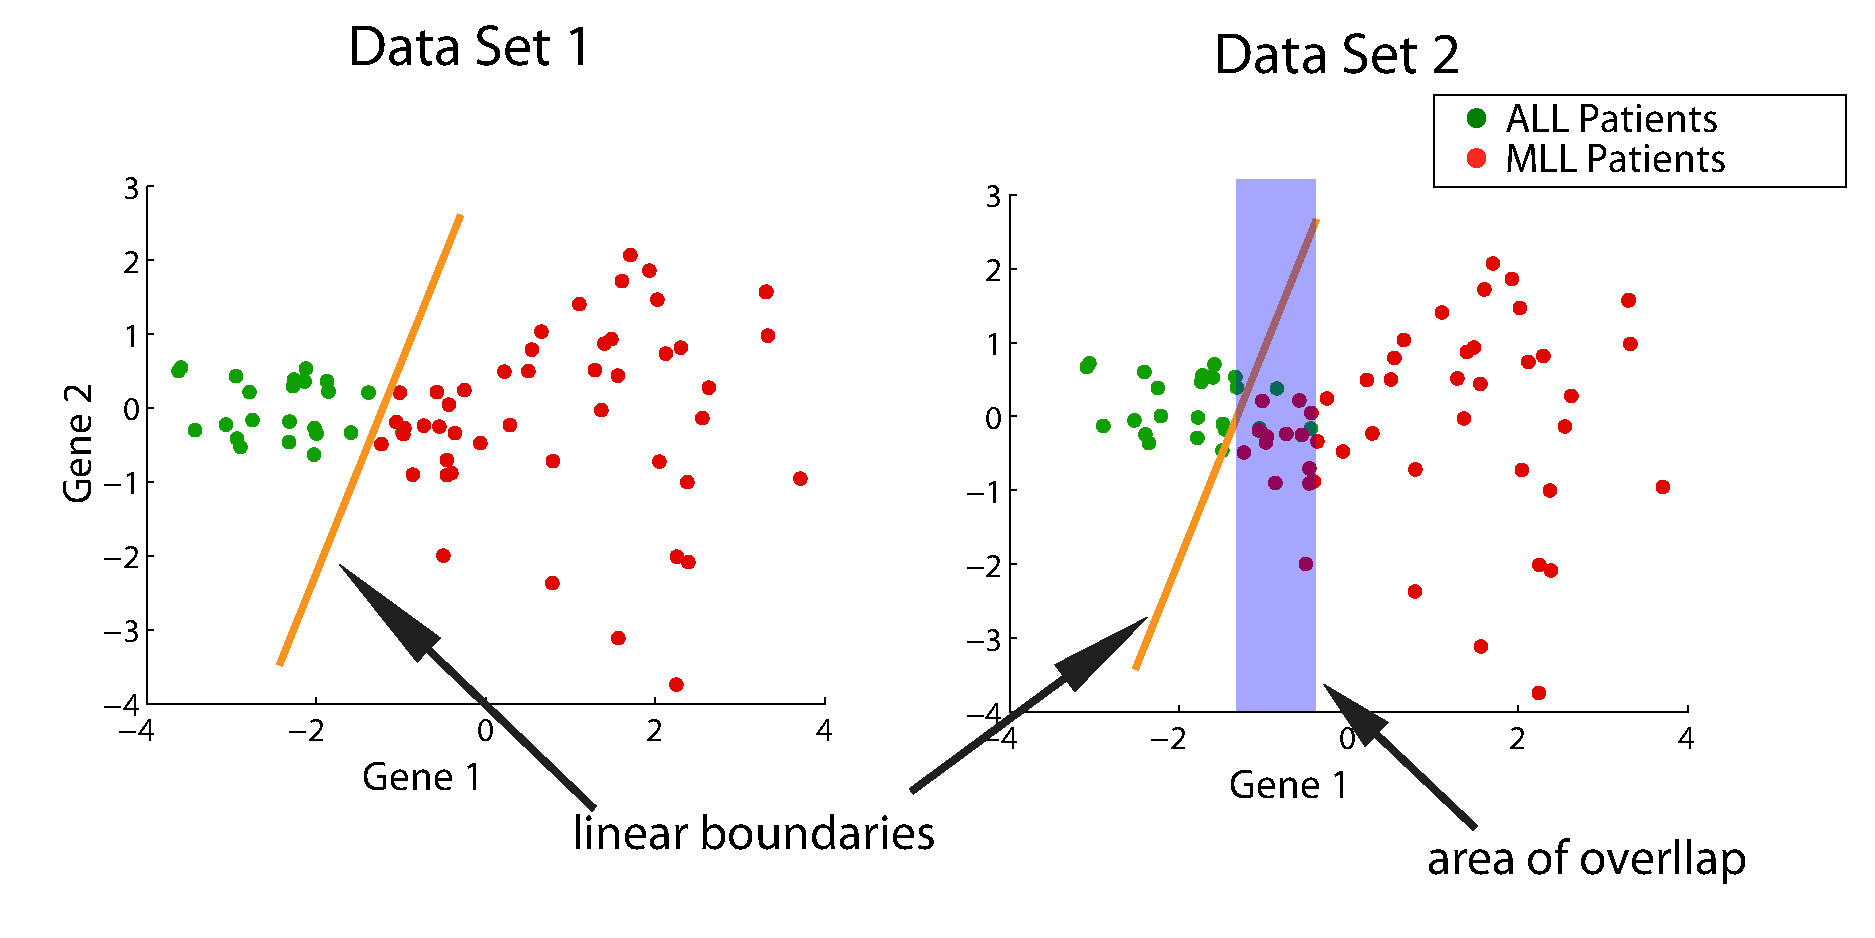
\includegraphics[width=1.0\columnwidth]{figs/complexity}}
\end{figure}

\subsection*{Figure 2 - Correlation between classification methods and complexity indices}

Scatter plot of complexity indices versus classification test errors
for different combinations of classification and feature selection
methods.  At each plot, points represent the 85 one-against-all
decompositions of the data sets. For each method, {\tt 1} stands for
no feature selection, {\tt 2} for BSS/WSS and {\tt 3} for Fisher
ratio. Numbers in the left upper corner of each scatter plot
correspond to the correlation between the error rate and complexity
indices, red values indicates correlations that are statistically
significant ($t$-test with $p$-value $< 0.01$).

\begin{figure}
\centerline{ 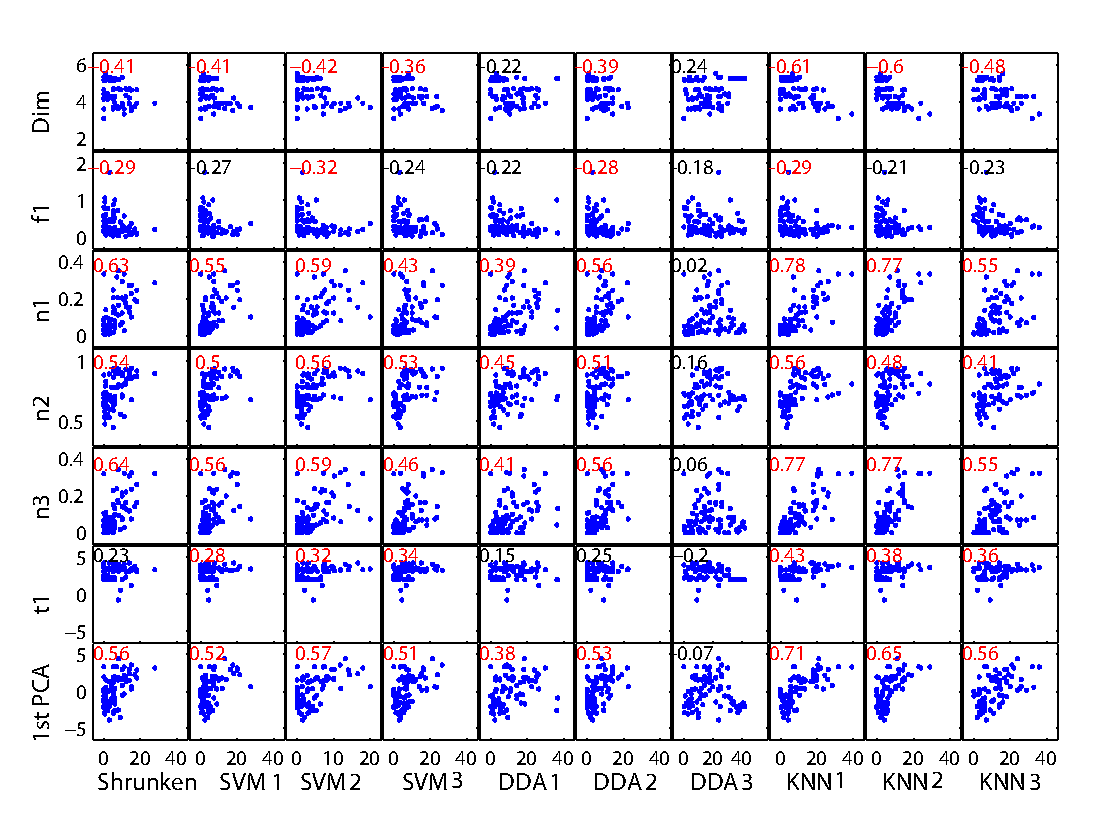
\includegraphics[width=1.0\columnwidth]{figs/indices}}
\end{figure}

%%%%%%%%%%%%%%%%%%%%%%%%%%%%%%%%%%%
%%                               %%
%% Tables                        %%
%%                               %%
%%%%%%%%%%%%%%%%%%%%%%%%%%%%%%%%%%%

%% Use of \listoftables is discouraged.
%%
\section*{Tables}

\subsection*{Table 1 - Data set description}
\begin{table*}[htp]
%\caption{Data Set Description}
\label{datasete}
\begin{center}
\begin{footnotesize}
\begin{tabular}{llllllll}
  \hline
  \bf{Dataset} & {\bf Chip} & \bf{\it{n}} & \bf{Dist. Classes} & \bf{\it{d}}\\
  \hline
{\tt Armstrong-V2}~\cite{Armstrong2002} & Affy & 72 & 24,20,28 & 2194 \\
{\tt Bhattacharjee}~\cite{Bhattacharjee2001} & Affy & 203 & 139,17,6,21,20 & 1543 \\
{\tt Chowdary}~\cite{Chowdary2006} & Affy & 104 & 62,42 & 182 \\
{\tt Dyrskjot}~\cite{Dyrskjoet2003} & Affy & 40& 9,20,11 & 1203 \\
{\tt Golub-V2}~\cite{Golub1999} & Affy & 72 & 38,9,25 & 1877 \\
{\tt Gordon}~\cite{Gordon2002} & Affy & 181 & 31,150 & 1626 \\
{\tt Laiho}~\cite{Laiho2007c} & Affy & 37 & 8,29 & 2202 \\
{\tt Nutt-V1}~\cite{Nutt2003}& Affy & 50 & 14,7,14,15 &  1377\\
{\tt Pomeroy-V1}~\cite{Pomeroy2002} & Affy & 34 & 25,9 & 857 \\
{\tt Ramaswamy}~\cite{Ramaswamy2001} & Affy & 190 & 11,10,11,11,22,10,11,10,30,11,11,11,11,20 & 1363 \\
{\tt Shipp}~\cite{Shipp2002} & Affy & 77 & 58,19 & 798 \\
{\tt Singh}~\cite{Singh2002b} & Affy & 102 & 58,19 & 339 \\
{\tt Su}~\cite{Su2001} & Affy & 174 & 26,8,26,23,12,11,7,27,6,28 & 1571 \\
{\tt West}~\cite{West2001} & Affy & 49 & 25,24 & 1198\\
{\tt Yeoh-V1}~\cite{Yeoh2002} & Affy & 248 & 43,205 & 2526 \\
{\tt Alizadeh-V1}~\cite{Alizadeh2000} & cDNA & 42 & 21,21 & 1095 \\
{\tt Alizadeh-V2}~\cite{Alizadeh2000} & cDNA & 62 & 42,9,11 & 2093 \\
{\tt Bittner}~\cite{Bittner2000}   & cDNA & 38 &  19, 19 & 2201 \\
{\tt Bredel}~\cite{Bredel2005} & cDNA  & 50 &   31,14,5 & 1739 \\
{\tt Chen}~\cite{XinChen06012002}  &   cDNA  & 180 &   104,76 & 85 \\
{\tt Garber}~\cite{Garber2001}  & cDNA &  66  &  17,40,4,5 & 4553 \\
{\tt Khan}~\cite{Khan2001}  & cDNA  & 83  & 29,11,18,25 & 1069 \\
{\tt Lapoint-V2}~\cite{Lapointe2004} & cDNA  &  110 & 11,39,19,41 & 2496 \\
{\tt Liang}~\cite{Liang2005} &   cDNA & 37 & 28,6,3 & 1411 \\
{\tt Risinger}~\cite{Risinger2003b} & cDNA & 42 & 13,3,19,7 & 1771 \\
{\tt Tomlins-V1}~\cite{Tomlins2007} & cDNA  & 104 &  27,20,32,13,12 & 2315 \\

% {\tt Armstrong-V1}~\cite{Armstrong2002} & Affy & Blood & 72 & 2 & 24,48 & 12582& 1081 \\
% {\tt Golub-V1}~\cite{Golub1999} & Affy & Bone marrow & 72 & 2 & 47,25 & 7129 & 1877 \\
% {\tt Nutt-V2}~\cite{Nutt2003} & Affy & Brain & 28 & 2 & 14,14 & 12625 & 1070 \\
% {\tt Nutt-V3}~\cite{Nutt2003} & Affy & Brain & 22 & 2 & 7,15 & 12625 & 1152 \\
% {\tt Pomeroy-V2}~\cite{Pomeroy2002} & Affy & Brain & 42 & 5 & 10,10,10,4,8 & 7129 & 1379 \\
% {\tt Yeoh-V2}~\cite{Yeoh2002} & Affy & Bone marrow & 248 & 6 & 15,27,64,20,79,43 & 12625 & 2526 \\
% {\tt Alizadeh-V3}~\cite{alizadeh00j} & cDNA & Blood & 62 & 4 & 21,21,9,11 & 4022 & 2093 \\
% {\tt Lapointe-V1}~\cite{Lapointe2004} & cDNA  &  Prostate &  69 &  3 &  11,39,19 & 42640 & 1625 \\
% {\tt Tomlins-V2} ~\cite{Tomlins2007} &  cDNA &    Prostate & 92 &  4 &   27,20,32,13 &  20000 & 1288 \\
\hline
\end{tabular}
\end{footnotesize}
\end{center}
We list the data sets and their characteristics such as type of
microarray chip (Chip), number of samples (n), distribution of samples
within the classes (Dist. Classes) and dimensionality (\it{d}).
\end{table*}






%%%%%%%%%%%%%%%%%%%%%%%%%%%%%%%%%%%
%%                               %%
%% Additional Files              %%
%%                               %%
%%%%%%%%%%%%%%%%%%%%%%%%%%%%%%%%%%%

\section*{Additional Files}
  \subsection*{Additional file 1 --- Table with Classification Error, Number of Selected Genes and Complexity Indices}

We present here a table with the classification error, number of selected genes and complexity indices against all data set decompositions. The data sets names corresponds to the descriptions in Table~1 and complexity indices and methods to the nomenclature from Figure~2. 



\end{bmcformat}
\end{document}





